\section{Introduction}
\label{intro}


\newcommand{\xidx}{i}
\newcommand{\yidx}{j}
\newcommand{\xw}[1]{w_{#1}}
\newcommand{\yw}[1]{w'_{#1}}

\cel{Start with a general statement of the research trajectory, then explain why we chose DP and Divide-and-Conquer as an example.}

% inductive :> PL, ML
% deductive :> proof (deductive), transformational

Software synthesis, the process of turning high-level specifications into executable, efficient
program code, has been a subject for research for about 30 years, yielding a wide range of techniques
and approaches. These can be roughly sorted into ``inductive'' approaches, which utilize concrete
values and execution traces, and ``deductive'' approaches, employing symbolic reasoning and treating
programs as composable mathematical objects.

While the former contains many techniques that make heavy use of solvers\marginpar{\tiny Sketch, Leon\ldots},
The latter relies mostly on theorem proof assistants such as Isabelle/HOL and Coq.
In a framework developed by Manna and Waldinger \marginpar{\tiny (e.g. 1980, 1992)}, the specification
is stated as a logical goal to be proven. The program is than read by interpreting the proof via the Curry-Howard
correspondance (also known as ``proofs-as-programs''). \newterm{Transformational} approaches\marginpar{\tiny KIDS/Specware, Spiral, AutoBayes, and also Fiat},
by contrast, maintain a knowledge base of valid transformations that are used to gradually refine a
specification down to the level of detail required to execute it.

While we stage our approach within the transformational synthesis camp, we strive to adopt factors
that contributed to the success of inductive synthesis over the past few years. In particular,
a high level of automation has been achieved thanks to the use of SAT and SMT solvers. These are used
to generate parameters and for checking candidate solution against the input specification.
We strive to harness their strength in a deductive setting, where 
\begin{itemize}
  \item The solver can directly check that a program term is equivalent to another term,
    thus merging branches and reducing repetitive manual labor.
  \item The solver can prove validity of side conditions that ensure the soundness of each individual
    transformations. This allows the construction of a library of \newterm{tactics} that can effect
    many kinds of transformations. The tactics gain more freedom and can be designed to be much more
    generic than if they were purely symbolic, since they do not have to represent logically valid
    equivalences: instead, they can represent equalities that are {\bf sometimes} true, and carefully
    check each context in which they are applied.
\end{itemize}


\begin{figure*}[b]
\centering
\resizebox{.9\textwidth}{!}{\begin{tikzpicture}[>=latex,mark options={scale=.5}]
	\begin{axis}[
	    ymode=log,
		xlabel=Problem size,
		ylabel=Time ({\it s}),
		scaled x ticks=false, %{real:1000}
		log basis y=2, ymajorgrids=true]
	\addplot[color=blue!50!white,ultra thick,mark=*,smooth] table[x=n/Time(s),y=COZ] {data/perf-gap.txt}
	  node(COZ-curve) [coordinate,pos=0.9] {};
	\addplot[color=orange!70!white,ultra thick,mark=*,smooth] table[x=n/Time(s),y=CO] {data/perf-gap.txt}
	  node(CO-curve) [coordinate,pos=0.8] {};
	\addplot[color=olive!70!white,ultra thick,mark=*,smooth] table[x=n/Time(s),y=LOOPDP] {data/perf-gap.txt}
	  [yshift=-12pt] node[pos=0.05] {LOOPDP};
	\addplot[color=red!70!white,ultra thick,mark=*,smooth] table[x=n/Time(s),y=Bellmania] {data/perf-gap.txt}
	  node(Bellmania-curve) [coordinate,pos=0.85] {};
	\end{axis}
	
	\begin{scope}[anchor=west]
	  \node(CO-lbl)[orange!80!white] at(2,1.5) {CO\_Opt};
	  \node(Bellmania-lbl)[red!80!white] at(1.5,1) {Bellmania};
	  \node(COZ-lbl)[blue!80!white] at(1.25,.5) {COZ};
	\end{scope}
	\begin{scope}[->,dashed]
	  \draw[orange] (CO-lbl) -- (CO-curve);
	  \draw[red] (Bellmania-lbl) -- (Bellmania-curve);
	  \draw[blue] (COZ-lbl) -- (COZ-curve);
	\end{scope}
\end{tikzpicture}

}
\caption{\label{intro:performance}
  Comparison of the the best performance obtained using polyhedral compilers 
  (PluTo\,\cite{HPC10/Pouchet}, PoCC\,\cite{PLDI08/Bondhugula})
  for parallelization, vs. manually crafted recursive divide-and-conquer implementations (CO),
  taken from~\cite{IPDPS15/Tithi}.}
\end{figure*}


\todo{Refactor so ``Divide and conquer DP'' occurs hear}
As a playground\coa{for loss of a better word?} in which to test and demonstrate our approach,
we explore the domain of divide-and-conquer dynamic programming algorithms.
Dynamic Programming (DP) algorithms build optimal solutions to a problem by combining
together optimal solutions to many overlapping subproblems.  DP
algorithms exploit this overlap to explore otherwise exponential-sized
problem spaces in polynomial time, making them central to many
important applications ranging from logistics to computational
biology. A recent textbook \cite{DurbinEdKr98} on biological sequence analysis, for example,
lists 11 applications of DP in bioinformatics in its introductory
chapter with many more in chapters that follow.


Dynamic programs are usually described through recurrence relations
that specify how the cells in a DP table must be filled up
using solutions already computed for other cells, but recent research has shown that it is possible
to achieve order-of-magnitude performance improvements over this
standard implementation approach by developing \emph{divide-and-conquer}
 implementation strategies that recursively
partition the problem into smaller subproblems.  These strategies
exhibit better temporal locality, and the partitioning can expose more
optimization opportunities (see, e.g., \cite{IPDPS15/Tithi}). 
Even when compared with tiled implementations optimized by the best polyhedral compilers, 
the divide-and-conquer implementations still show significantly better performance, in some cases
by more several orders of magnitude as illustrated in \Cref{intro:performance}. 

Developing such implementations, however, is quite difficult, as will become apparent in \Cref{divide}.
In this paper, we develop a new computer aided approach to formally deriving provably correct divide-and-conquer algorithms
for dynamic programming problems. The approach relies on a new method to formalize the derivation of these algorithms, which
allows an algorithm designer to guide the derivation process through a small number of very high-level tactics. 
Specifically, our paper makes the following contributions\coa{Move earlier?}:
\begin{enumerate}
  \item We develop a small set of formal \newterm{solver-aided tactics} that can be used to transform a class of recurrence
  specifications, written in a simple functional language, 
  into equivalent divide-and-conquer programs, that admit parallel cache-local
  implementations, in a principled, systematic manner.
  \item We prove that these tactics are semantics-preserving, assuming some side conditions are met
  at the point when the tactic is applied.
  \item We show that the side conditions can be effectively translated into first-order closed
  formulas, and verified automatically by SMT solvers.
\end{enumerate}


\section{Divide and Conquer DP}
\label{divide}

As a motivating example, we consider the Simplified Arbiter problem.
Two processes $x$ and $y$ are scheduled to run $|x|$ and $|y|$ time slots,
respectively. Execution starts at $t=0$, and the length of each time slot is
one time unit. The cost for scheduling the slots $[a..b)$ of $x$ at $t=a+c$
is given by $\xw{abc}$, and the cost for schedulting the slots $[a..b)$ of $y$
at same $t=a+c$ is given by $\yw{abc}$.

\begin{figure}
\begin{tabular}{@{\hspace{-1pt}}r@{~}l@{}}
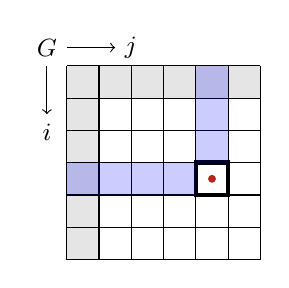
\begin{tikzpicture}[x=4.1mm,y=4.1mm,baseline=(center), remember picture]
  \coordinate(center) at (3,3);
  \draw[step=1] (0,0) grid (6,6);
  \draw[ultra thick] (4,2) rectangle +(1,1);
  %\node(Gij) at (4.5,2.5) {\tiny $\scriptscriptstyle\langle i,j\rangle$};
  \node[circle,fill=BrickRed,inner sep=0,minimum size=1mm](Gij) at (4.5,2.5) {};
  \fill[black,opacity=0.1] (0,5) rectangle (6,6);
  \fill[black,opacity=0.1] (0,0) rectangle (1,5);
  \fill[blue,opacity=0.2] (0,2) rectangle (4,3);
  \fill[blue,opacity=0.2] (4,3) rectangle (5,6);
  \node[anchor=south east](G) at (0,6) {\small$G$};
  \draw[->] (G.east) -- +(1.5,0) node[anchor=west] {\small $j$};
  \draw[->] (G.south) -- +(0,-1.5) node[anchor=north] {\small $i$};
\end{tikzpicture}
&
\small
$
\begin{array}{l@{}}
	\tikz[overlay, remember picture]{\draw[BrickRed] (0,0) -- (Gij);}
	G_{ij} ~=~ \\
	~
	\begin{cases}
		0                        & i=j=0 \\
		\yw{0j0}                  & i=0, j>0 \\
		\xw{0i0}                 & i>0, j=0 \\
		\begin{array}{@{}l@{\hspace{-1pt}}l@{\hspace{-4pt}}}
		  \min\langle & \underset{0\leq q<j}\min ~ G_{iq} + \yw{qji},  \\
		              & \underset{0\leq p<i}\min ~ G_{pj} + \xw{pij}~\rangle
		\end{array}              & i,j>0
	\end{cases}
\end{array}
$
\end{tabular}
\vspace{5pt}
\caption{Recurrence equation and cell-level dependencies.}
\label{intro:arbiter spec}
\end{figure}


The optimal cost for scheduling the first $i$ slots of $x$ and the first $j$ slots
of $y$ is given by the recurrence in \Cref{intro:arbiter spec}. When $i$ is zero, it means that
only $y$ has been scheduled, so the cost is $\yw{0j0}$, and similarly when $j$ is zero, 
the cost is $\xw{0i0}$. When $i$ and $j$ are both positive, there are two options:
either the schedule ends with an allocation to $x$, 
where slots $[p..i)$ of $x$ were scheduled at $t=p+j$, and the cost is 
$G_{pj} + \xw{pij}$; or it ends with an allocation to $y$, where
slots $[q..j)$ of $y$ were scheduled at $t=i+q$, and the cost is $G_{iq} + \yw{qji}$.
The minimum over all respective $p<i$ and $q<j$ is taken.
Eventually, the optimal cost of the entire schedule is given by $G_{|x||y|}$.

\begin{paragraph}{Iterative Algorithm.}
Using a standard dynamic programming method, Richard, an algorithms expert, computes this recurrence
with an iterative program by understanding the dependency pattern:
to compute the $\min\langle\rangle$ expression in \Cref{intro:arbiter spec} and find the optimal
values for $p$ and $q$, the algorithm needs information from all cells above and to the left of $G_{ij}$.
In particular, each value $G_{ij}$ is computed from other values $G_{i'j'}$ with lower
indexes, $i'<i$, ~$j'<j$. 
Therefore, considering $G$ as a two-dimensional array, it can be filled in a single pass from left to right and from top
to bottom.
\end{paragraph}

\newcommand\FORLINE[1]{\STATE\algorithmicfor~{#1} \algorithmicdo~}

\begin{algorithm}
\renewcommand\arraystretch{1.3}
\begin{algorithmic}
  \STATE $G_{00} := 0$
  \FORLINE{$j=1..|y|$}  $G_{0j} := \yw{0j0}$  
  \FOR{$i=1..|x|$}
    \STATE $G_{i0} := \xw{0i0}$
    \FOR{$j=1..|y|$}
      \STATE $G_{ij} :=
        \begin{array}[t]{@{}l@{~}l} 
          \min\langle & \underset{0\leq q<j}\min ~ G_{iq} + \yw{qji}, \underset{0\leq p<i}\min ~ G_{pj} + \xw{pij}~\rangle \\         
        \end{array}$
    \ENDFOR
  \ENDFOR
\end{algorithmic}
\caption{\label{intro:iterative}
   Iterative Simplified Arbiter}
\end{algorithm}


\newcommand\qbox[1]{\fbox{\scriptsize#1}}

\begin{paragraph}{Divide-and-Conquer Algorithm.}

\begin{figure}
\centering
\begin{tabular}{c@{\hspace{.5in}}c}
$
\renewcommand\arraystretch{2}
\begin{array}[b]{c|c|c|c|}
  \multicolumn{2}{c}{} & \multicolumn{2}{c}{J} \\ \cline{3-4}
  \multicolumn{2}{c}{} & \multicolumn{1}{c}{J_0}  & \multicolumn{1}{c}{J_1}\\ \cline{3-4}
  \multirow{2}{*}{$I$} & I_0 & 1 & 2 \\ \cline{3-4}
    & I_1 & 3 & 4 \\ \cline{3-4}
\end{array}
$
& 
$\begin{array}[b]{l}\qbox1 \rightsquigarrow \qbox2 \\ 
\qbox1 \rightsquigarrow \qbox3 \\ \qbox2\rightsquigarrow \qbox4 \\ \qbox3 \rightsquigarrow \qbox4\end{array}$
\end{tabular}
\vspace{5pt}
\caption{\label{intro:quadrants}
  Dividing a two-dimensional array into quadrants; the dependencies are shown on the right.}
\end{figure}

Divide-and-conquer is an algorithm development pattern (\cite{SODA06/Chowdhury}, \cite{SPAA08/Chowdhury})\coa{should these (SODA/SPAA) be the ones to cite here?}, 
where the DP table is partitioned into regions, and each region is expressed as a sub-problem
to be solved.

In our case, Richard takes the two-dimensional array $G$ and partitions it into
quadrants, as illustrated in \Cref{intro:quadrants}. He then applies the same reasoning
as in the iterative case, concluding that the computations of 2 and 3 depend on 1,
and the computation of 4 depends on 2 and 3.
\end{paragraph}

Richard \emph{stratified} the computations on these quadrants into the following
four steps:
\begin{algorithmic}[1]
  \STATE Compute \qbox1 (using only input data $w,w'$).
  \STATE Compute \qbox2 using data from \qbox1.
  \STATE Compute \qbox3 using data from \qbox1.
  \STATE Compute \qbox4 using data from \qbox2 and \qbox3.
\end{algorithmic}

Each step depends only on a subset of the steps that came before it, 
as illustrated by \Cref{intro:chain}. However, this is not yet a divide-and-conquer algorithm: 
of the four steps, only step \qbox1{} is an instance of the original problem; all the other steps
look somewhat different from the original problem and lack significant locality. With some algebraic manipulation, however, 
it is possible to define each of the four steps above recursively, leading to a true divide-and-conquer algorithm with very high locality 
and significantly improved performance relative to the iterative algorithm.

To illustrate how this is done, we first introduce a small amount of notation. 
We define $I$ and $J$ to be the index sets for the rows and columns, respectively.
We then define partitions $I=I_0\cup I_1$ and $J=J_0\cup J_1$ as in \Cref{intro:quadrants}.
$G$ is now parameterized on those index sets;

\begin{equation}
\begin{array}{l@{}l}
	G^{^{IJ}}_{(i:I)\,(j:J)} ~=~  \\
	\qquad
	\begin{cases}
		0                         & i=j=0 \\
		w_{0j0}                   & i=0, j>0 \\
		w'_{0i0}                  & i>0, j=0 \\
		\begin{array}{@{}l@{~}l}
		  \min\langle & \underset{q\in J\cap[0,j)}\min ~ G^{^{IJ}}_{iq} + \yw{qji}, \\
		              & \underset{p\in I\cap[0,i)}\min ~ G^{^{IJ}}_{pj} + \xw{pij}~\rangle
		\end{array}              & i,j>0
	\end{cases}
\end{array}
\end{equation}

The computation of \qbox1 corresponds to computing $G^{IJ}$ within the sub-domain 
$I_0\times J_0$, making it an exact copy of $G^{I_0J_0}$. This is due to the fact
that for $j\in J_0$, ~$J\cap[0,j)=J_0\cap[0,j)$, and for $i\in I_0$, ~$I\cap[0,i)=I_0\cap[0,i)$.

On the other hand, the computation of \qbox2 is {\bf not} a mere copy of $G^{I_0J_1}$, 
because the range $q\in J\cap[0,j)$ is not a subset of $J_1$, so that
some of the recursive references $G_{iq}$ are outside of \qbox2.

This can be addressed by splitting that range, adding yet range another parameter to $G$.

\begin{equation}\LeftEqNo
\begin{array}{l@{}l}
	G^{^{IJJ'}}_{(i:I)\,(j:J)} ~=~  \\
	\qquad
	\begin{cases}
		0                         & i=j=0 \\
		w_{0j0}                   & i=0, j>0 \\
		w'_{0i0}                  & i>0, j=0 \\
		\begin{array}{@{}l@{~}l}
		  \min\langle & \underset{~q\in J'~}\min ~ G^{^{IJ'\!J'}}_{iq} + \yw{qji}, \\
		              & \underset{q\in J'\cap[0,j)}\min ~ G^{^{IJJ}}_{iq} + \yw{qji}, \\
		              & \underset{p\in I\cap[0,i)}\min ~ G^{^{IJJ'}}_{pj} + \xw{pij}~\rangle
		\end{array}              & i,j>0
	\end{cases}
\end{array}
\end{equation}

The computation of \qbox2 is now a copy of $G^{I_0J_1J_0}$. ~$G$ can be further generalized in the following
way:

\newcommand{\Ggen}{H}

\begin{equation}\LeftEqNo
\begin{array}{l@{}l}
	\Ggen^{^{IJ}}_{(i:I)\,(j:J)\,\psi} ~=~  \\
	\qquad
	\begin{cases}
		0                         & i=j=0 \\
		w_{0j0}                   & i=0, j>0 \\
		w'_{0i0}                  & i>0, j=0 \\
		\begin{array}{@{}l@{~}l}
		  \min\langle & \psi_{ij}, \\
		              & \!\underset{q\in J\cap[0,j)}\min ~ G^{^{IJJ}}_{iq} + \yw{qji}, \\
		              & \!\underset{p\in I\cap[0,i)}\min ~ G^{^{IJJ}}_{pj} + \xw{pij}~\rangle
		\end{array}              & i,j>0
	\end{cases}
\end{array}
\label{intro:Ggen}
\end{equation}

It is easy to see that both $G$ and \qbox1 can be expressed in terms of $\Ggen^{IJ}$ by making $\psi_{ij}=\infty$, 
but more importantly, \qbox2 can now also be expressed in terms of $\Ggen^{I_0J_1}$ by making 
$\psi_{ij} =  \underset{q\in J_0}\min ~ G^{I_0J_0J_0}_{iq} + \yw{qji}$.
Moreover, the calls to $G$ inside $\Ggen$ can be replaced with recursive calls to $\Ggen$ itself,
giving the form: 

\begin{equation}\LeftEqNo
\begin{array}{l@{}l}
	\Ggen^{^{IJ}}_{(i:I)\,(j:J)\,\psi} ~=~  \\
	\qquad
	\begin{cases}
		0                         & i=j=0 \\
		w_{0j0}                   & i=0, j>0 \\
		w'_{0i0}                  & i>0, j=0 \\
		\begin{array}{@{}l@{~}l}
		  \min\langle & \psi_{ij}, \\
		              & \!\underset{q\in J\cap[0,j)}\min ~ H^{^{IJ}}_{iq} + \yw{qji}, \\
		              & \!\underset{p\in I\cap[0,i)}\min ~ H^{^{IJ}}_{pj} + \xw{pij}~\rangle
		\end{array}              & i,j>0
	\end{cases}
\end{array}
\end{equation}

The same approach can be used to develop the computations of \qbox3 and \qbox4.
The sub-computation of $\psi$ can also be transformed into four recursive sub-computations, further improving the locality of the resulting algorithm.
So through these kind of transformations, it is possible to break the computation of the original $G$ into four (or more) subcomputations, each of which can be itself recursively partitioned into four subcomputations, giving us a true divide-and-conquer algorithm.
When the pieces become small enough, the iterative algorithm (\Cref{intro:iterative}) is executed.

\medskip
As was outlined in \Cref{intro}\coa{check the ref, I suspect it is going to move}, prior work has shown that the performance results that can be achieved through these transformations can be dramatic. Unfortunately, the line of reasoning that was followed in this section can get quite complicated for most dynamic programming algorithms, and producing a correct divide-and-conquer algorithm for a given dynamic programming problem is considered quite difficult even by the researchers who originally pioneered this technique. 

In the following sections, we describe the parts that make Bellmania --- a formal framework for deriving algorithms from specifications. 
It utilizes \newterm{solver-aided tactics} to generate provably correct pseudo-code; 
this approach is demonstrated by engineering specialized tactics for the domain of divide-and-conquer DP.


\begin{figure}
\centering
\begin{tikzpicture}[>=latex,x=6mm,y=6mm,
    every path/.style={step=1},
    every node/.style={inner sep=.5pt},
    block/.style={rectangle,draw,thick,fill=blue, fill opacity=0.15, inner sep=0}]
    
  \def\dx{1.75cm}
  \def\w{3mm}
    
  \draw (0,0) grid (2,2);
  \node(1) at (.5,1.5) {1};   \node(2) at (1.5,1.5) {2};
  \node(3) at (.5,.5) {3};    \node(4) at (1.5,.5) {4};

  \node[inner sep=0] at (2.5,1) {
\includegraphics[width=\w]{img/arrow}};

  \tikzset{xshift=\dx}
  
  \draw (0,0) grid (2,2);
  \node(1) at (.5,1.5) {\,1$'$};   \node(2) at (1.5,1.5) {2};
  \node(3) at (.5,.5) {3};         \node(4) at (1.5,.5) {4};
  \node(s)[block,fit={(0,1) (1,2)}] {};
  \node[inner sep=0] at (2.5,1) {
\includegraphics[width=\w]{img/arrow}};

  \tikzset{xshift=\dx}
  
  \draw (0,0) grid (2,2);
  \node(1) at (.5,1.5) {\,1$'$};  \node(2) at (1.5,1.5) {\,2$'$};
  \node(3) at (.5,.5) {3};        \node(4) at (1.5,.5) {4};
  \draw (s.70) edge[->,out=20] (2);
  \node(s)[block,fit={(0,1) (1,2)}] {};
  \node[inner sep=0] at (2.5,1) {
\includegraphics[width=\w]{img/arrow}};

  \tikzset{xshift=\dx}
  
  \draw (0,0) grid (2,2);
  \node(1) at (.5,1.5) {\,1$'$};   \node(2) at (1.5,1.5) {\,2$'$};
  \node(3) at (.5,.5) {\,3$'$};    \node(4) at (1.5,.5) {4};
  \draw (s.south) edge[->,out=-40,in=-150] (3.250);
  \fill[block] (0,0) |- (.92,1) to[out=0,in=-90] (1,1.08) |- (2,2) |- (1.08,1) to[out=180,in=90] (1,.92) |- cycle;
  \coordinate(s) at (.8,0);
  \node[inner sep=0] at (2.5,1) {
\includegraphics[width=\w]{img/arrow}};

  \tikzset{xshift=\dx}

  \draw (0,0) grid (2,2);
  \node(1) at (.5,1.5) {\,1$'$};   \node(2) at (1.5,1.5) {2$'$};
  \node(3) at (.5,.5) {\,3$'$};    \node(4) at (1.5,.5) {4$'$};
  \draw (s.south) edge[->,out=-30,in=-150] (4);
  
\end{tikzpicture}
%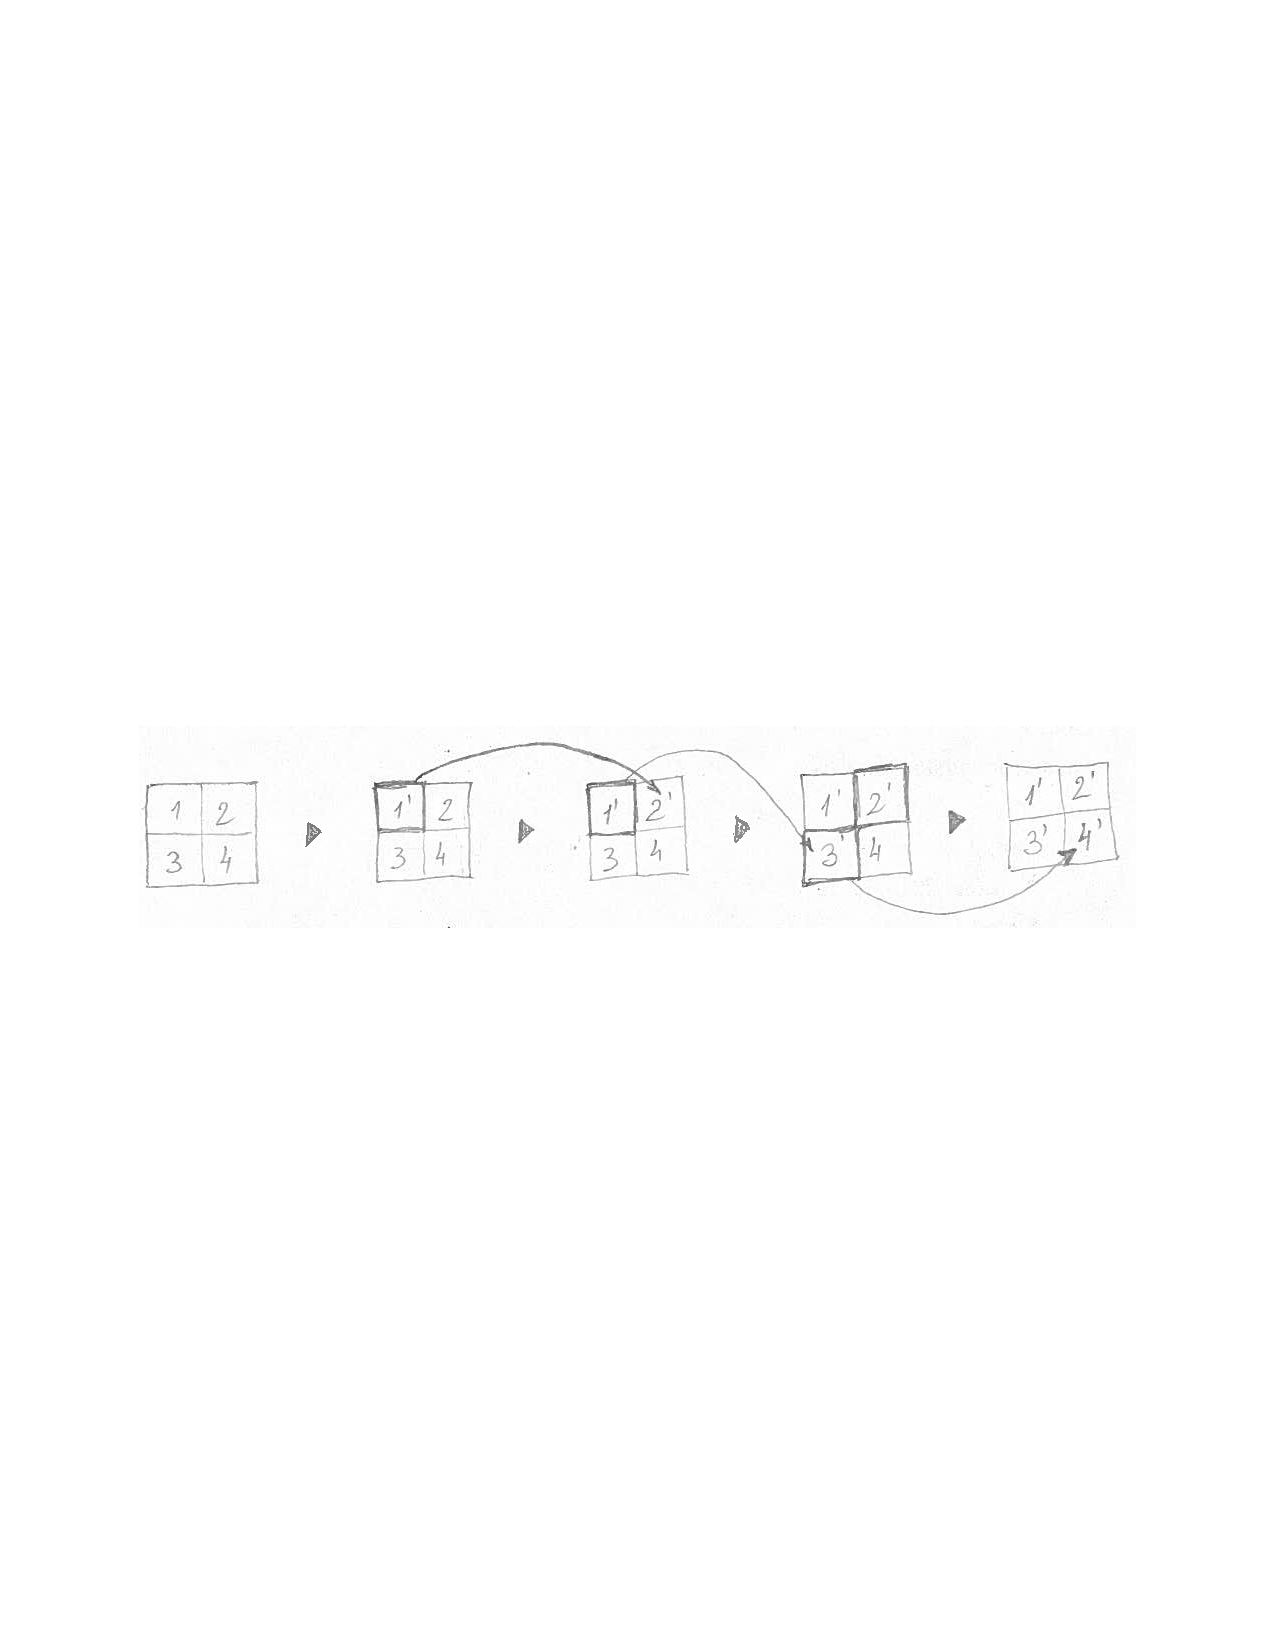
\includegraphics[width=.47\textwidth]{img/gap-stratify1}
\caption[caption]{\label{intro:chain}
  Stratified computation for Simplified Arbiter. \\[.2em]
  Shaded areas indicate the region that is read at each step.}
\end{figure}


